\documentclass{article}
\usepackage[T1]{fontenc}
\usepackage{geometry}
\geometry{a4paper}
\usepackage{setspace}
\usepackage{enumerate}
\usepackage{enumitem}
\usepackage{hyperref}
\usepackage[toc]{glossaries}
\hypersetup{colorlinks,allcolors=black,urlcolor=blue}

\setenumerate[1]{itemsep=0pt,partopsep=2pt,parsep=0pt ,topsep=2pt}
\setitemize[1]{itemsep=0pt,partopsep=2pt,parsep=0pt ,topsep=2pt}
\setenumerate[2]{itemsep=0pt,partopsep=2pt,parsep=0pt ,topsep=2pt}
\setitemize[2]{itemsep=0pt,partopsep=2pt,parsep=0pt ,topsep=2pt}
\setdescription{itemsep=0pt,partopsep=2pt,parsep=0pt ,topsep=2pt}

\usepackage{graphicx}
\usepackage{fontspec}

\defaultfontfeatures{%
	RawFeature={%
		% +swsh,
		+calt
	}%
}

\setmainfont{EB Garamond}

\usepackage{multicol}
\usepackage{float}

\usepackage[semibold]{sourcecodepro}

\usepackage{xcolor}
\usepackage{minted}
\usemintedstyle{friendly}

\definecolor{bg}{rgb}{0.95,0.95,0.95}
\newcommand{\codeinline}[1]{
	\mintinline[bgcolor=bg, fontsize=\scriptsize]{text}{#1}
}


\usepackage{relsize}
\newcommand{\bigdataVs}[1]{
	\subsection{#1}
}

\newenvironment{console}{% Caution:
	\VerbatimEnvironment
	\begin{minted}[xleftmargin=2em,bgcolor=bg,fontsize=\small]{console}% Do NOT delete these comments
	}% Otherwise there will be error when compiling
	{%
	\end{minted}%
}

%-----------%

\title{NoSQL Proof-of-Concept Proposal -- Dota2 Game Replay Analysis}
\author{
	Team name: PSG.LGD \\ \\
	Yichun Yan \\
	Ziwei Jiang \\
	Yifan Li \\
	Weiqi Wang
}
\date{\today}


\makeglossaries


\newglossaryentry{Ancient}
{
    name={Ancient},
    description={(also commonly refered to as Thrones, or Tree for Radiant's ancient and Throne for Dire's ancient, as legacy names from DotA) are massive structures found inside each faction's base and are the main objective. In order to win, the enemy team's Ancient must be destroyed, while the own one must be kept alive. Ancients are guarded by their two tier 4 towers. The Ancients are invulnerable until both of their tier 4 towers are destroyed.}
}
\newglossaryentry{MOBA}
{
    name={MOBA},
    description={also known as action real-time strategy (ARTS), is a subgenre of strategy video games that originated as a subgenre of real-time strategy in which each player controls a single character, usually on a map in an isometric perspective, as part of a team competing against another team of players.}
}
\newglossaryentry{professional matches}
{
    name={professional matches},
    description={Matches played two professional teams hosted officially by Valve.}
}
\newglossaryentry{public matches}
{
    name={public matches},
    description={Matches played by ten randomly chosen players, and the results won't influence Matchmaking Rating(MMR) of each player.}
}
\newglossaryentry{ranked matches}
{
    name={ranked matches},
    description={Matches played by ten randomly chosen players according to their Matchmaking Rating(MMR), and the results will influence the Matchmaking Rating of each player.}
}
\newglossaryentry{gold}
{
    name={gold},
    description={Gold is the currency used to buy items or instantly revive your hero. Gold can be earned from killing heroes, creeps, or buildings.}
}
\newglossaryentry{creeps}
{
    name={creeps},
    description={Creeps are basic units in Dota 2. Every unit which is not a hero, building, ward or courier is considered a creep. Creeps can belong to either faction, be neutral, or be player-controlled units. Unlike heroes, creeps do not gain experience and cannot level up. All of their stats are set values (though can still be altered by modifiers). Most creeps grant a set gold and experience bounty to heroes when killed.}
}
\newglossaryentry{XP}
{
    name={XP},
    description={A shorthand for experience. Experience is an element heroes can gather by killing enemy units, or being present as enemy units get killed. On its own, experience does nothing, but when accumulated, it increases the hero's level, so that they grow more powerful. Only heroes can gather experience and therefore reach higher levels. With each level gained, a hero's base attributes increase by static values (unique for each hero), which makes them stronger in several.}
}
\newglossaryentry{match id}
{
    name={match id},
    description={A unique identifier for each match played on Dota2.}
}
\newglossaryentry{sequence number}
{
    name={sequence number},
    description={Similar to match id, which is a unique identifier for each match. But this field will not show up in the Dota2's client.}
}
\newglossaryentry{towers}
{
    name={towers},
    description={Towers are the main line of defense for both teams, attacking any non-neutral enemy that gets within their range. Both factions have all three lanes guarded by three towers each.}
}
\newglossaryentry{barracks}
{
    name={barracks},
    description={Barracks (commonly shortened to Rax) are buildings, defended by their tier 3 towers, that are responsible for keeping lane creeps as powerful as their counterparts.}
}
\newglossaryentry{lane}
{
    name={lane},
    description={A Lane is one of three paths connecting the two Ancients. Lane creeps will push along these lanes after spawning.}
}
\newglossaryentry{AFK}
{
    name={AFK},
    description={A shorthand for away-from-keyboard, AFK means a player leaving a match early before it's end.}
}
\newglossaryentry{buff}
{
    name={buff},
    description={Buffs are positive status effects that enhance your hero.}
}
\newglossaryentry{debuff}
{
    name={debuff},
    description={Debuffs are negative status effects that weaken your hero.}
}
\newglossaryentry{mode}
{
    name={mode},
    description={Game modes are a set of restrictions within which the game of Dota 2 can be played. Most game modes alter how heroes are picked by players. There are also some novelty modes that allow 1v1 play, or give a player a new hero every time they die, for example. }
}
\newglossaryentry{ban}
{
    name={ban},
    description={A ban will disallow the choose for a specific hero within a match.}
}
\newglossaryentry{pick}
{
    name={pick},
    description={A pick is choosing a hero that a player want to play within a match.}
}
\newglossaryentry{first-blood}
{
    name={first-blood},
    description={The first kill within a game. The player who makes the first kill will be rewarded with 150 extra gold}.
}
\newglossaryentry{team battle}
{
    name={team battle},
    description={A battle involves more than half of the players in a match within a short period of time}.
}
\newglossaryentry{buyback}
{
    name={buyback},
    description={While dead, the player has the option to use ``buyback", spending money in order to instantly respawn at the fountain. However, the buyback ability has a long cooldown of 480 seconds and has a scaling gold cost.}.
}
\newglossaryentry{last-hit}
{
    name={last-hit},
    description={You can only get gold from killing creeps or get a kill from killing a hero if you make the last-hit that cause the creeps or hero to death.}.
}
\begin{document}

\maketitle

\tableofcontents
\clearpage

%-------%

\section{Project Background}

Our team aims at exploring data about a popular and long-lived computer game, Dota2. Dota2 is a multiplayer online battle arena (\gls{MOBA}) video game developed and published by Valve Corporation. Each game will involves ten players that are divided to two teams play against each other on a same map. Every player chooses one ``hero" that has unique abilities and different styles of playing. The aim for each team is to destroy the building called ``\gls{Ancient}" of the other team. Players collect \gls{gold} to buy powerful items and gain \gls{XP} by killing players on the other team, destroy building of the other team, or kill \gls{creeps}.

\begin{figure}[H]
	\centering
	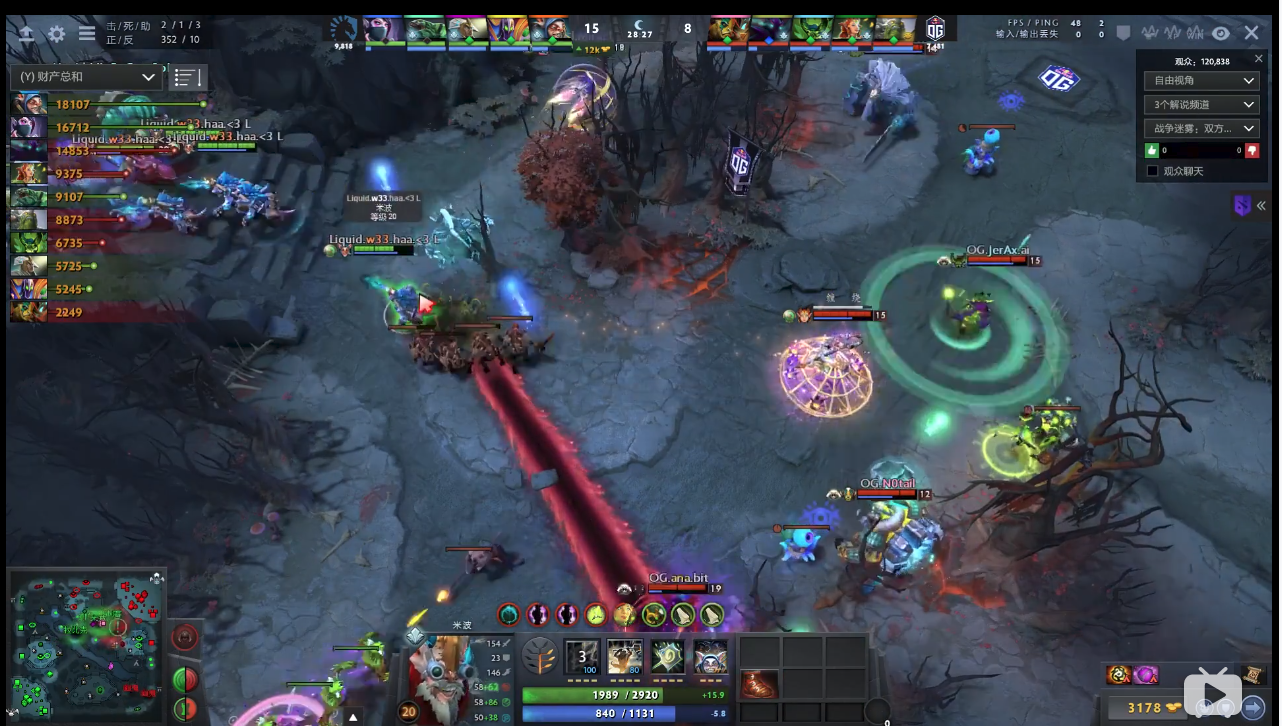
\includegraphics[width=\linewidth]{pic/combat.png}
	\caption{A screenshot of the game}
\end{figure}
This game has a large quantity of players, accordingly a huge amount of replays will be produced every day. Also, it's a real-time game, hundreds of operations and some decisions will be made each second, and all of them will have some influence on the final results of the game. Both of the above two features make the game a great subject to big data analysis. Actually, there are some professional teams start hiring data engineers to help their players perform better in a game. This means that our analysis has some realistic meaning.

Knowing that this game is not familiar to everybody, and we may use some words that may be difficult to understand to those who don't play this kind of games for simplicity. I create a glossary at the end of this proposal for your reference.
\section{Potential Datasets}
We will mainly use two datasets:

\begin{enumerate}
\item \href{https://wiki.teamfortress.com/wiki/WebAPI/GetMatchDetails}{Dota2 match result dataset}
\item \href{https://wiki.teamfortress.com/wiki/Replay}{Dota2 replay dataset}
\end{enumerate}

The first dataset is the snapshot of the final state of each player and the whole game, containing only important information.
The second one is a binary format file which can be executed by Dota2's client to reproduce everything happened in the game.

The datasets can be retrieved from the following resources:

\begin{enumerate}
\item Valve's Dota2 replay servers
\item \href{https://wiki.teamfortress.com/wiki/WebAPI}{Valve's official API}
\end{enumerate}

We will get the match results data from Valve's official API.
It also provides a key, which we can use to retrieve a replay from the replay server.

In all, we will have two different kinds of data for our further analysis, relatively large-scale but coarse-grained match results data, and very fine-grained replays data.
Considering the file size of one replay, we decide to include recent professional games and randomly select some public games for the replay data.
We will mention how we acquire the data in Data ETL section.

\section{Five Vs of Datasets}

To assess the adequacy of adopting big data to our project, we firstly identify five Vs characteristics of our dataset.

\bigdataVs{Volume}

Replays are one of the datasets we plan to use, which are the full records of finished matches. The size of one replay is estimated to be about 60MB. We plan to collect 3000 replays whose size is about 180GB. As for match result data which is JSON-format data, the size of each result is about 5KB. We plan to collect 10,000,000 match results whose size is about 50GB. Moreover, if we desire more data in future implementation, we can always access it as long as Dota2 still has players.

\bigdataVs{Velocity}

According to the statistic data in August 2019 from Steam which is a video game digital distribution platform, the average number of players is 467,148.3 players and the peak number is 826,690.
A large number of players makes both the replay data and result data high-velocity.
Although in our project, the velocity depends on the velocity of the API request, this statistic data reveals that it's potential to be high-velocity.

\bigdataVs{Variety}

From the APIs mentioned above, we can access JSON format files, the match result data, and binary format files, the replay data.

\bigdataVs{Veracity}

The overall quality of our datasets is good because we access most of them from the official API.
But there is still a few noises.
For example, the time of some games is too short, which makes these game lack of representativeness.
Thus, we plan to implement data validation to filter the undesired matches.

\bigdataVs{Value}

Dota2 game statistics and replays data are valuable.
Professional teams may use it to analyze the performance of team members or design new strategies for competitions.
Amateur players can also learn a lot about the techniques, timing, hero choice from the data.
Our business questions, will focus on these aspects to provide valuable insights.

Even though the game is versioning, our datasets can be useful for a relatively long time.
Because we plan to collect 1/3 \gls{professional matches} and 1/3 \gls{public matches}, 1/3 \gls{ranked matches}.
The professional matches are durable since we can always extract information about professional teams and players from them.
As for the public games, they are valuable as long as they are not too stale. Minor changes of the game does not affect the whole picture.
But we will filter out public games which are too outdated in the data validation step, in order to make our datasets more valuable.

\section{Potential Business Questions}

As mentioned before, we can collect 2 kinds of data, one is match results and one is replays.
By analyzing them, the following questions might be answered.

\begin{itemize}
    \item Easy questions:
    \begin{itemize}
        \item Who is the hero gaining \gls{gold}/\gls{XP} fastest in 15 minutes in public games/professional games?
        \item Who is the hero having most kills/assists/heals/deaths in \gls{public matches}/\gls{ranked matches}/\gls{professional matches}?
        \item What is the most purchased item in \gls{public matches}/\gls{ranked matches}/\gls{professional matches}?
        \item Who is the hero having most bad-manner players (players who are \gls{AFK} or disconnected)?
        \item Who is the most popular hero (the hero who has the highest pick rate) in \gls{public matches}/\gls{ranked matches}/\gls{professional matches}?
        \item Who is the hero having the highest ban rate in \gls{professional matches}?
        \item who is the hero having the most \gls{ban}/\gls{pick} rate in \gls{professional matches}?
        \item How long does a game cost on average in \gls{public matches}/\gls{ranked matches}/\gls{professional matches}?
        \item Which item is used most in \gls{public matches}/\gls{ranked matches}/\gls{professional matches}?
    \end{itemize}
    We categorize these questions as easy questions because the solutions to them are straight-forward. These questions can be answered by implementing aggregation on our datasets. And most of the data needed for these questions can be extracted directly from our datasets.
    \\

    \item Moderately challenging questions:
    \begin{itemize}
        \item How are the benefits gained from \gls{buyback}s in \gls{public matches}/\gls{ranked matches}/\gls{professional matches}?
        \item How is the vision in \gls{public matches}/\gls{ranked matches}/\gls{professional matches}?
        \item When does the first team battle happen in \gls{public matches}/\gls{ranked matches}/\gls{professional matches}?
        \item Which is lineup having the highest win rate in \gls{public matches}/\gls{ranked matches}/\gls{professional matches}?
        \item Which is the most popular lineup (lineup which has the highest pick rate) in \gls{public matches}/\gls{ranked matches}/\gls{professional matches}?
        \item Which is the most common ban-pick combo in \gls{public matches}/\gls{ranked matches}/\gls{professional matches}?
        \item Who is the hero changed most in win/\gls{pick}/\gls{ban} rate after releasing a new version of Dota2?
        \item Who is the hero having the highest winning rate in each \gls{lane}?
    \end{itemize}
    We categorize these questions as moderately challenging questions because the solutions to them are not that straight-forward as easy questions. The first challenge is to define some terms we used in these questions in the application code. For example, we use the term, vision, which is involved with the lifecycle of ward and sentry (two items provide visibility around them). Besides aggregation, we also need join operations to answer these questions.\\

    \item Challenging questions:
    \begin{itemize}
        \item How is the winning-losing relationship between Dota2 professional teams? Can we use a graph to visualize it?
        \item Does there exist a regular farming path for some professional players?
        \item Does there exist a correlation between the time of the \gls{first-blood} and the time of the entire game?
        \item Does there exist a correlation between the \gls{gold}/\gls{XP} source of a hero and its win rate?
        \item Does there exist a correlation between the distribution of the economy and the result of the game?
        \item Does there exist a correlation between economic development and the time of the first \gls{team battle}?
    \end{itemize}
    We categorize these questions as challenging questions because they need more techniques than moderately challenging questions. Like moderately challenging questions, they have some ambiguous definition needs to be implemented. But they cannot be answered easily by aggregation and join operations. Instead, we plan to use machine learning techniques to solve them.
\end{itemize}


\section{Data ETL}

\subsection{Extraction}

Valve, the company that develops the game, initially try to provide all the players with easy APIs to access the data of the game.
But due to the increasing stress on its data servers, many of its APIs are shut down.
At the same time, the documentation seems to be never updated since it's created, which makes it much more difficult for us to collect the data.
For example, the API which returns a bunch of the match results given a starting match id is not usable anymore.
Another API which returns a key that is critical for construct the URL to download replay of that game is not working as well.

But luckily, we found some hints from the \href{https://dev.dota2.com}{developer's forum of Dota2}.
We can use the starting \gls{sequence number}, which works similarly as the \gls{match id}, to get a series of game results.
And by calling a third party API from OpenDota, we can get the important key to constructing the URL to download replays again.

The specific steps of gaining our data are as following:

\begin{enumerate}
\item Match Results:
	\begin{itemize}
		\item Use \href{https://wiki.teamfortress.com/wiki/WebAPI/GetMatchHistoryBySequenceNum}{GetMatchHistoryBySequenceNum} API to get the match ids. We will need a a field called \\ \codeinline{start_at_match_seq_num} to specify the starting match sequence number of the results.
		\item Then we can extract the last sequence number of the results as the \codeinline{start_at_match_seq_num} for the next call. By doing this iteratively we can enlarge our dataset for our first kind of data.
	\end{itemize}
\item Replays:
	\begin{itemize}
		\item Get the match ids of recent professional games from the last step.
		\item Use the those ids via \href{https://docs.opendota.com/#tag/matches}{OpenDota API} to get the information we need \\ (\codeinline{cluster} and \codeinline{replay_salt}) for retrieving replays from Valve's replay server
		\item Construct links in this format:\\  \codeinline{ http://replay<cluster>.valve.net/570/<match_id>_<replay_salt>.dem.bz2} to get the replays.
	\end{itemize}
\end{enumerate}


\subsection{Transformation}

The match result is in JSON format so we can almost directly store it. The information it contains is:

\begin{itemize}
	\item Players information:
	\begin{itemize}
		\item Account id
		\item Player slot
		\item The hero he uses in this match
		\item The items he possesses at the end of the match
		\item The player's kills/deaths/assists
		\item The player's leaver status (whether \gls{AFK}/disconnected or not)
		\item The gold he possesses at the end of the match
		\item The amount of \gls{last-hit}s and denies the player got during the match
		\item The average \gls{gold}/\gls{XP} he gained per minute
		\item The total gold he spent during the match
		\item The amount of damage the player dealt to heroes/\gls{towers}
		\item The amount of health the player had healed on heroes
		\item The player's level at match end
		\item A list detailing a player's ability upgrades, including the ability and the upgrading time
		\item Additional playable units owned by the player and its items
	\end{itemize}
	\item The season the game was played in
	\item The winner team of the match
	\item The length of the match
	\item Unix timestamp of when the match began
	\item The matches unique ID
	\item A sequence number, representing the order in which matches were recorded
	\item The tower status of both teams
	\item The \gls{barracks} status of both teams
	\item The server cluster the match was played upon
	\item The time in seconds since the match began when \gls{first-blood} occurred
	\item The \gls{mode} of the match
	\item The number of human players within the match
	\item The league that this match was a part of
	\item The number of thumbs-up/thumbs-down the game has received by users
	\item A list of the picks and bans in the match, if the game \gls{mode} is Captains Mode
\end{itemize}


On the other hand, the replay data is completely unstructured \codeinline{.dem.bz2} binary file,
data transformation must be done before we can store the data in our database.

Firstly, we can decompress the \codeinline{.bz2} file with \codeinline{org.apache.commons.compress.compressors.bzip2} package in Java,
which will give us a \codeinline{.dem} file:

Next, we can utilize \href{https://github.com/skadistats/clarity}{clarity},
an open source Dota2 replay parser, to extract useful information from the \codeinline{.dem} file.

It cannot be achieved by a single click, though. We have to write a lot of code to invoke its function.
What's more, clarity does not provide detailed documentation, instead there are only some \href{https://github.com/skadistats/clarity-examples}{examples} which forces us to iteratively attempt and learn the usage of this tool.

Based on our exploration, the following data will be available:

\begin{itemize}
	% info
	\item Player name, id, team formation and hero choice
	% combatlog
	\item Detailed log of the game, including a hero:
	\begin{itemize}
		\item deals damage to another one
		\item heals another one
		\item receives/loses a \gls{buff}/\gls{debuff}
		\item kills another one
		\item uses his ability
		\item uses an item
		\item buys an item
		\item receives/loses some \gls{gold}
		\item gains some \gls{XP}
		\item buys back (spending money in order to instantly re-spawn)
	\end{itemize}
	% lifestate
	\item Spawn/death of heros and NPCs
\end{itemize}

These information will be organized in a Document and store to our database.

Most fields in our datasets are related to some of the above-mentioned business questions.
They are all important.
We will generally validate them, for example, fields like the HP, XP, total gold cannot be negative.

What's more important is to filter out invalid data on the game level. Some of the games lasts for only two or three minutes, because some players are disconnected and others just quit the game very quick. Others are practicing games where most players are computer bots. We will completely drop these game records.



% --------------------------------------------

% Except for those listed above:

% Run success but hard to find meaning:
% 	dump, dumpbaselines, dumpmana, gameevent, modifiers, particles
%	propertychange, resources, seek, spawngroups, stringtabledump, tick

% Run failed: allchat, livesource, metadata, serializers,

% Unknown:
%   - dtinspector: Seems to provide a GUI interface but I(LYF) run in docker, which raises an exception.
%	- entityrun: No output
%	- matchend: Produced result but also raises exception
%	- tempentities: No output

% --------------------------------------------

\subsection{Loading}

\subsubsection{NoSQL Storage Technology}

As we mentioned above, we have two datasets - one is the match results data in JSON format, which is a kind of document that can be encoded using a text-based encoding scheme.
The replay data is binary files which is inappropriate for document NoSQL database to store.
But after we parsing those replay data, we can gather useful information from replay data in Document format.

Therefore, we choose to use MongoDB as our primary NoSQL storage technology.

MongoDB is a popular NoSQL storage device that can store high volume, high velocity, high variety Big Data datasets.
It's a document storage device, which makes storing semi-structured document-oriented data such as JSON much easier.
It is an open-source NoSQL database, so we are free to use it.

Also, MongoDB supports partial update.
This will help us aggregate values in future games that we would potentially use.

To answer the business question about the relationship between professional teams and players, using only MongoDB may involve considerable aggregations. We may consider using a graph database, neo4j, as our secondary NoSQL technology choice.

\subsubsection{Docker}

In order to combine different needs, programming languages and developing environment of many technologies, we will adopt Docker to our project.
Using Docker, we can deploy our application into any environment.

Docker is a container technology that provides consistency.
It's open-source and there are many open source applications that have been made in \href{https://hub.docker.com}{Docker Hub}.
Docker Hub provides official or verified images, so it's safe to use.

In our project, we will build Dockerfile to let it connect with our project.
We will use Scala as programming language, and we will get the match results data from Dota2's official API.
MongoDB will be used as database. And then we will put all of this into a Docker container.

\subsubsection{AWS (Amazon Web Service)}

As we mentioned before, we need 50GB to store the JSON file, and we need 180GB to store replay data, and the scale would be extended if we add more data in the datasets.
In order to have enough capacity to store datasets, we will use AWS (Amazon Web Server) to deploy our project on a cloud server.
Running Docker on AWS will provide us an open-source and free way to build and run a distributed application and provide a reliable and easy way to scale out.

AWS provides numbers of official ways to deploy docker on AWS, such as Amazon ECS, which is a highly scalable, high-performance container orchestration service to run Docker containers on the AWS cloud.
After we package datasets and analytics packages into Docker, we will deploy Docker to Amazon ECS.

%-------%

\section{Overview of our Architecture}

\begin{figure}[H]
	\centering
	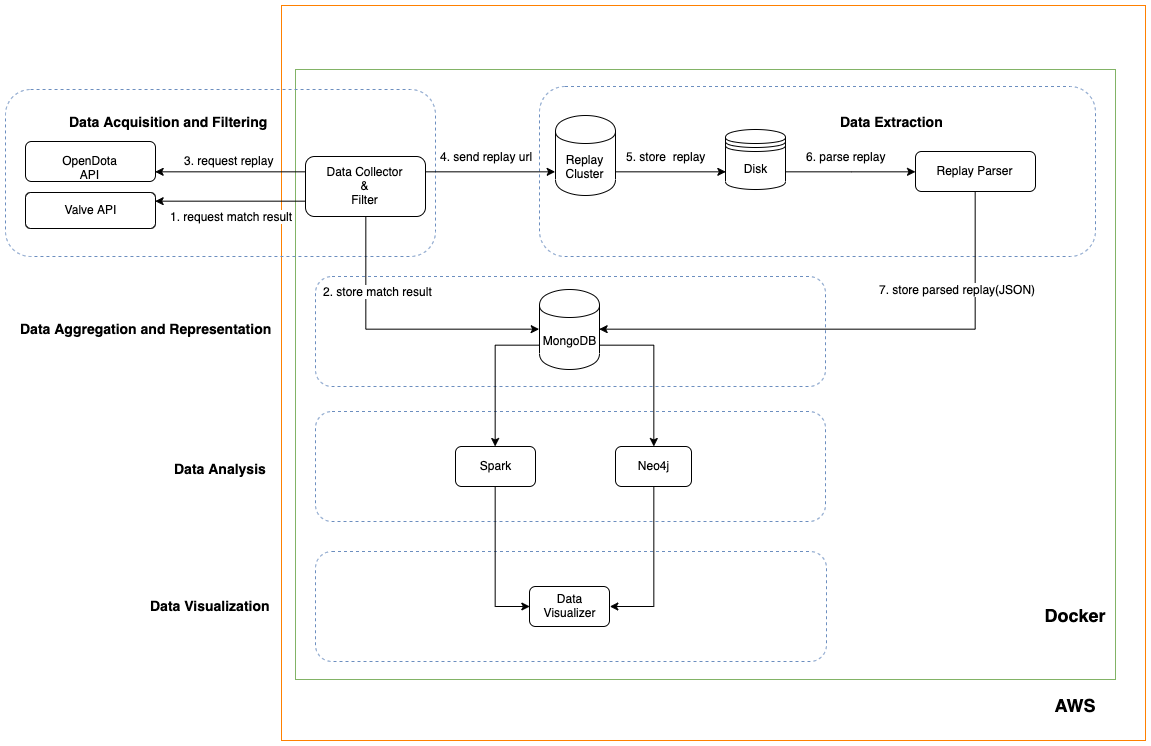
\includegraphics[width=\linewidth]{pic/arc.png}
	\caption{Our Project's Structure}
\end{figure}

\section{Potential Challenges}

There are several aspects where we may have potential challenges.

During the environment setup:

\begin{itemize}
	\item We are trying to build a docker containerized application, but none of our team members have previous experience
	\item We do not have experience about using AWS or other cloud services, neither
\end{itemize}

In the data ETL phase:

\begin{itemize}
	\item Download replays from the server can be slow, the links may not work
	\item Professional games are relatively rare, so more efforts will be needed to find and retrieve the professional replays
	\item Both APIs have call limits, even though we can control our request frequency, some request may still fail
	\item Some downloaded replay files may be broken so that no information can be extracted, or they may even cause exceptions in the pipeline
	\item The open-source replay parser does not have documentation, thus some of our parsing code may cause unexpected exceptions when there are some corner case
	\item Although we try our best to write the code to handle errors to avoid the program failing, but there still can be cases that are not covered, since our architecture involves a lot of network communications and i/o. We might need to design a log system to help us restore from a crash.
\end{itemize}


In the data analysis phase:

\begin{itemize}
	\item Lots of joins and aggregations between the two datasets will be involved
	\item We must quantitatively define some generally used concepts which are often qualitatively used, for example, the measurement of vision, team battle, etc. An inappropriate definition can make the whole conclusion meaningless
	\item When we are answering the relationship between the teams or players, we will have to extract and load the data to a secondary database, like neo4j
\end{itemize}

\printglossary

%-------%

\end{document}
